\subsection{Experiment 7: Noisy Handwritten Digits with Temperature Encoded Symbols} \label{sec:experiment-7}

\subsubsection{Objective}

In Section \ref{sec:theory-approach-methodology-temperature-encoding} we explained our observation of how humans learn to perform arithmetic. We explained how children in particular learn to represent digits by mapping between the image of a digit and the image of familiar objects. These familiar objects (like apples for example) behave as symbols that convey both quantity and ordinal relationships. The human learner can then act on these symbols to produce a more accurate result. This process allows the human learner to generalize the solution to combinations of digits that they have not experienced before.

We believe a neural network model can be constructed that learns in a similar way. The network is provided a sequence of handwritten digits and an operator symbol. It is trained to develop an internal representation that can map between the image of the digit and a symbol that captures both the quantity and ordinal relationships represented by the digit (the temperature encoded symbol). The model is also trained to perform the arithmetic operation on the two digits. With deep recurrent neural networks, these two related tasks can be combined into one model that can learn to perform both with high accuracy.

The purpose of this experiment is to show that it is indeed possible to build such a model and that the use of symbols represented as temperature encodings can improve the accuracy of training on a restricted dataset as well as force the learning algorithm to discover a representation that can generalize to unseen combinations of digits. We also investigate how varying the amount of symbols present affects the accuracy of the model on the unseen test data.

\subsubsection{Method}

Five recurrent neural network models are developed for this experiment each having the same architecture. Figure \ref{fig:sequential-model-noisy-temperature} shows a diagram of the architecture used. The models accept a sequence of four 28x28 images. The first two images are of the MNIST handwritten digit operands, the third image is the operator (plus, minus, times and divide) consistently rendered in a standard font, and finally the fourth image is an equals sign. The model is trained so that when it sees the operands on each of the first two time steps, it outputs a temperature encoded symbol that represents the digit in the image. When the model is presented with the operator on the input, it performs the operation on the operands and then outputs a temperature encoded symbol that represents the least significant digit of the result. Finally, when the equals sign is presented, the model outputs a temperature encoded symbol representing the most significant digit of the result.

The neural network architecture used is composed of an input layer of 784 units for the 28x28 pixel images. Two hidden layers are used each consisting of 512 LSTM units. The output layer is a vector of nine elements to represent the temperature encoded results. The networks are trained using the Adam optimizer with the mean square error as the loss function and a learning rate of 0.001. Training is performed over 200 epochs in batches of 100 and the model performing best on the validation set is saved.

\begin{figure}
	\centering
	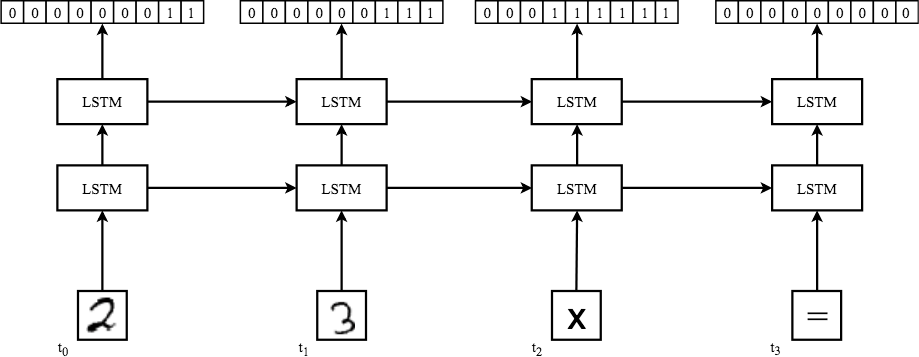
\includegraphics[max width=\textwidth]{sequential-model-noisy-temperature}
	\caption{A sequential model learning to perform arithmetic on images of handwritten digits in the presence of symbols. The symbols are provided on the outputs of the first two intermediate steps using temperature encoding. Here the model is performing multiplication on the combination: 2 x 3.}
	\label{fig:sequential-model-noisy-temperature}
\end{figure}

The same dataset used in Experiment 4 in Section \ref{sec:experiment-4} is also used for this experiment with the exception of replacing one-hot vector symbols with temperature encoded symbols. To recap, for each operator, the combinations of digits are split into a set of seen combinations that includes, 80\% of the combinations of digits. For each of the seen combinations, eight MNIST samples are selected. Four of these samples are used for training, two for validation and the remaining two for testing. The remaining 20\% of the combinations are reserved as the set of unseen combinations that are used to verify that the models have learned an algorithm of the operations. The dataset of seen combinations is replicated five times, each replica includes a different percentage of symbols present. The symbol spreads used are 0\%, 25\%, 50\%, 75\% and 100\%. The symbols were presented as output labels to the first two time steps. The model is trained to classify the handwritten digit with the aid of the symbol provided. When symbols are not provided, a vector composed of 0.5 dummy values is used instead. Each model is trained five times using 5-fold cross-validation.

\subsubsection{Results}

\begin{table}[p]
	\center
	\caption{A comparison of the mean accuracy and standard deviation along with the p-value of a hypothesis t-Test when compared to the 0\% symbols model when tested on the test set of \textbf{seen} combinations.}
	\label{tab:experiment-8-results-table-seen}
	\begin{tabular}{ |c|c|c|c| } 
		\hline
		\% Symbols Present & Accuracy (\%) & Standard Deviation  & p-value\\ 
		0\% & 41.55 & 0.0302 & NA \\  
		25\% & 51.30 & 0.0457 & 0.02311\\  
		50\% & 60.65 & 0.0379 & 0.00049 \\  
		75\% & 75.84 & 0.0587 & 0.00063\\  
		100\% & 84.26 & 0.0582 & 0.00018\\  
		\hline
	\end{tabular}
\end{table}

\begin{table}[p]
	\center
	\caption{A comparison of the mean accuracy and standard deviation along with the p-value of a hypothesis t-Test when compared to the 0\% symbols model when tested on the test set of \textbf{unseen} combinations.}
	\label{tab:experiment-8-results-table-unseen}
	\begin{tabular}{ |c|c|c|c| } 
		\hline
		\% Symbols Present & Accuracy (\%) & Standard Deviation  & p-value\\ 
		0\% & 4.62 & 0.0133 & NA \\  
		25\% & 25.53 & 0.0900 & 0.16889\\  
		50\% & 45.90 & 0.0319 & 0.00199 \\  
		75\% & 54.63 & 0.0324 & 0.0\\  
		100\% & 69.58 & 0.0694 & 0.00088\\  
		\hline
	\end{tabular}
\end{table}

\begin{figure}[p]
	\centering
	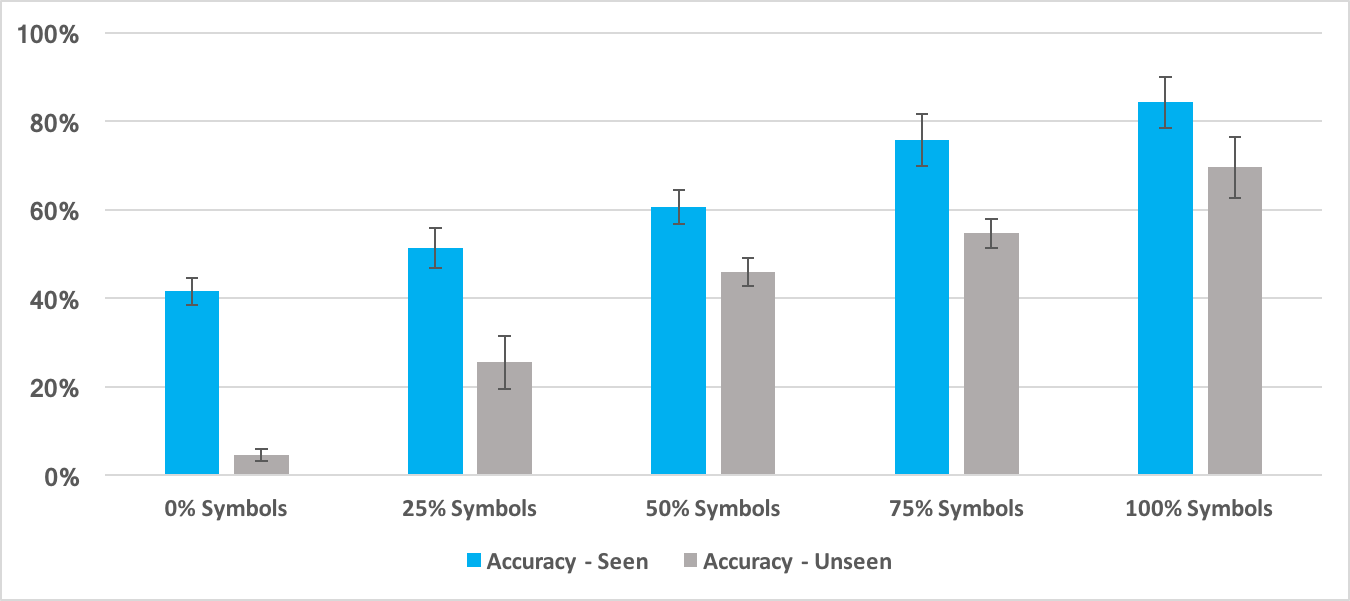
\includegraphics[max width=\textwidth]{experiment-8-results-chart-2}
	\caption{A comparison of the mean accuracy and 95\% confidence intervals for each of the models trained with 0\% to 100\% temperature encoded symbol presence when tested on both the test set of \textbf{seen} and \textbf{unseen} combinations.}
	\label{fig:experiment-8-results-chart}
\end{figure}

Table \ref{tab:experiment-8-results-table-seen} shows the results of testing the models on the test set of seen combinations. Similarly, Table \ref{tab:experiment-8-results-table-unseen} shows the results of testing the model on the test set of unseen combinations. The tables present the mean accuracy, standard deviation and the p-test score for each of the models developed. Figure \ref{fig:experiment-8-results-chart} depicts the mean accuracies along with the 95\% confidence intervals for all five models trained on both the seen and unseen test sets.

\subsubsection{Discussion}

The results show that increasing the number of symbols available per combination during training, improves the accuracy of the recurrent network when tested on combinations the model has seen during training. This result is comparable to Experiment 4 where we had a similar architecture and approach. However, we used a different representation for the symbols, namely temperature encoded vectors. More importantly the results show the accuracy on unseen combinations increases as more symbols are used during training. These results confirm the findings we've observed in several of our previous experiments and also supports our hypothesis that artificial neural networks similar to human learners can benefit from the presence of clear and concise symbols when training using limited datasets.

The results in this experiment show that the way the symbols are represented can have significant effect on the learning ability of the models. The one-hot vector representation was effective for learning a simple mapping function when all combinations of inputs were provided during training. However, it failed to capture the ordinal nature of the digits and therefore they were not able to discover a representation for an algorithm that can perform the arithmetic operations. By using temperature encoded symbols for the digits, the models are able to represent the arithmetic algorithm and generalize to unseen combinations of digits.